\section{Network configuration}
\label{sec:network_configuration}
The \jx has a built in ethernet adapter and has been equipped with an extra WiFi adapter, as well as a network card consisting of four independant ethernet adapters \cite[Section 6.5]{martensPortableSensorRig2022}.
The following section presents relevant iformation aboud network configuration and outlines the steps to achieve a bandwidth of $1Gb/s$ on each of the four Ethernet adapters.

\paragraph{Link-Local Addresses (LLA)} are a commonly used in \gls{gigev} camera setups \cite{teledyneSettingIPAddress01} \cite{lucidvisionlabsArenaSoftwareDevelopment2020}.
It enables devices to automatically be assigned IP addresses without a specific subnet without relying on a \gls{dhcp} server or static IP \cite{annieahujaweb2020LinkLocalAddress2022}.
This allows direct connection between a \gls{gigev} camera and an ethernet adapter without an intermediary router \cite{annieahujaweb2020LinkLocalAddress2022}.

As shown in Figure \ref{fig:lucid_ip_discovery}, the \cams are configured to use \gls{lla} if the use of Persistend IP and \gls{dhcp} fails \cite{lucidvisionlabsArenaSoftwareDevelopment2020}.
This is levraged during the discovery process as discussed in Section \ref{sec:discovery}.

\paragraph{Static IP} is supported by the \cams, but I decided not to use this feature \cite{lucidvisionlabsArenaSoftwareDevelopment2020}.
The motivation to avoid this was to avoid the need to change the IP ranges of the network adapters and to keep the cameras in their factory default configuration, as this would make it easier to use them for other projects in the future.

\paragraph{Jumbo Frames} is a type of network frame that carries more payload than the standard \gls{mtu} size \cite{ieeeIEEEStandardsInterpretation2002} \cite{lucidvisionlabsJumboFramesLUCID2020}.
Increasing the maximal \gls{mtu} size typically leads to improved performance for high-bandwidth cameras and can also help reduce the CPU load on the host system, as there is less protocol overhead \cite{lucidvisionlabsJumboFramesLUCID2020} \cite{lukeThingsYouShould2018}.
Both the ethernet card used on the \jx as well as the \cams support Jumbo frames \cite{IntelI350am4Chip} \cite{lucidvisionlabsTritonMPPolarized2020}.
To enable jumbo frames on a device the following command is used \code{ifconfig <device> mtu 9000}.

\begin{figure}[H]
    \centering
    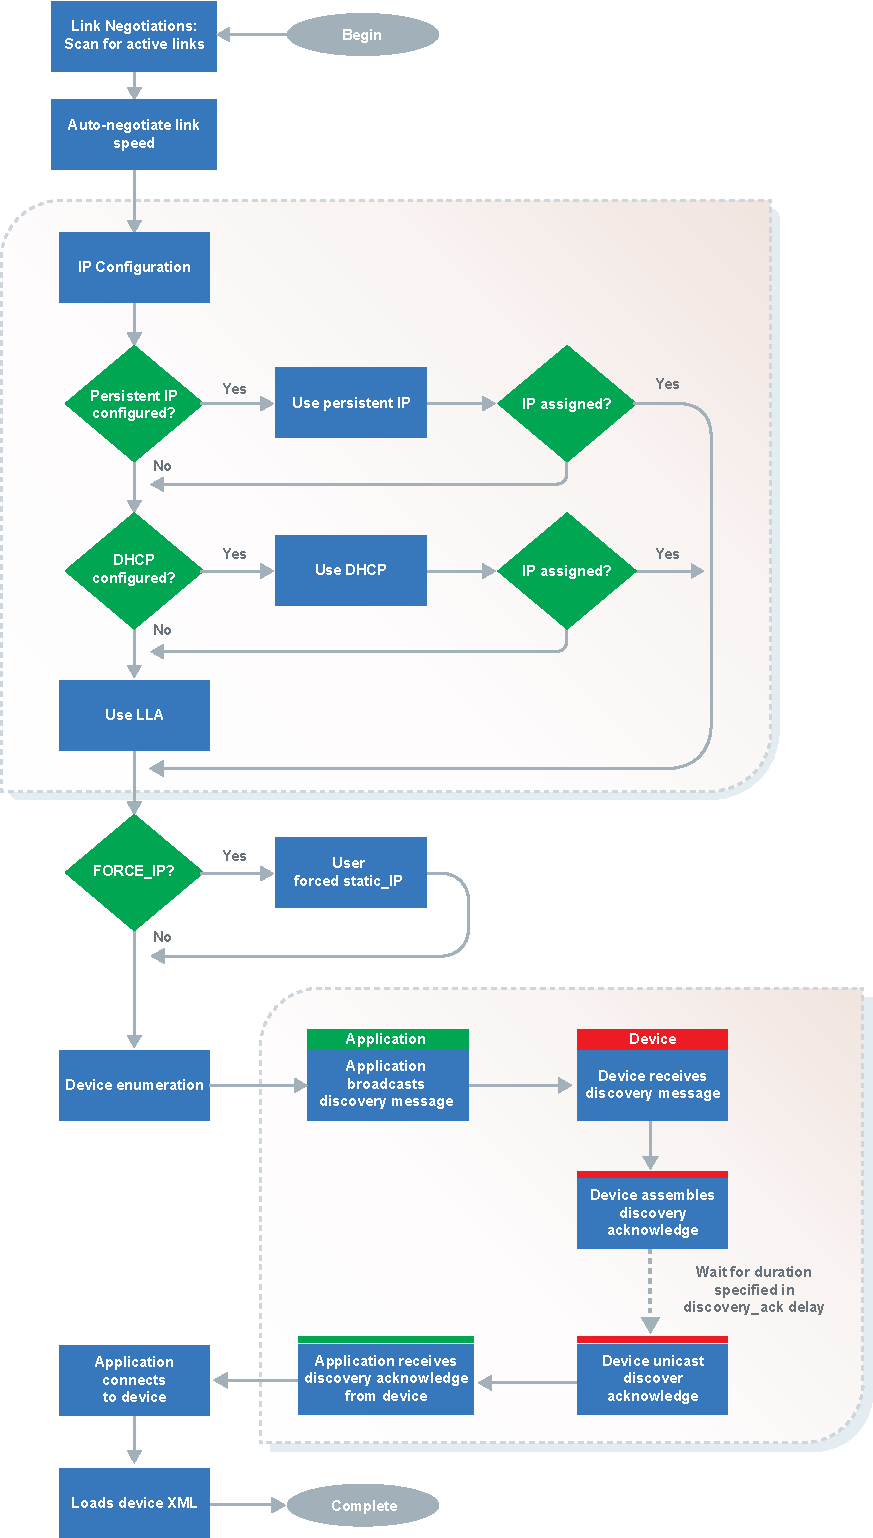
\includegraphics[height=\textheight]{figures/PDF/lucid_ip_discovery.pdf}
    \caption{Figure of the descovery and enumeration process of Lucid cameras \cite{lucidvisionlabsTritonMPPolarized2020}}
    \label{fig:lucid_ip_discovery}
\end{figure}


\paragraph{Receive Buffers} are storage areas where network packets are temporarily held before being processed by the \gls{cpu}, as depicted in Figure \ref{fig:linux_network} \cite{danQueueingLinuxNetwork2013}.
To enhance performance and prevent starvation, it is recommended to increase the default number of receive buffers, also known as \glspl{skb} \cite{lucidvisionlabsReceiveBuffers2020} \cite{danQueueingLinuxNetwork2013}.
On the \jx, the maximum number of receive buffers was raised from the default 256 to 4096 using the command \code{ethtool -G <device> rx 4096} \cite{danQueueingLinuxNetwork2013}.
Additionally, the maximum buffer size was permanently increased to $16MiB$ by adding the following lines to the \code{/etc/sysctl.conf} file \cite{redhat10ChangingNetwork}\cite{ibmIBMDocumentationTCPIP2021}:

\begin{minted}{bash}
net.core.rmem_default=16777216
net.core.rmem_max=16777216
\end{minted}

Expanding the number of buffers increases memory usage and may introduce additional latency as the queue grows longer, but in this case, it did not lead to any issues \cite{danQueueingLinuxNetwork2013}.

\begin{figure}[H]
    \centering
    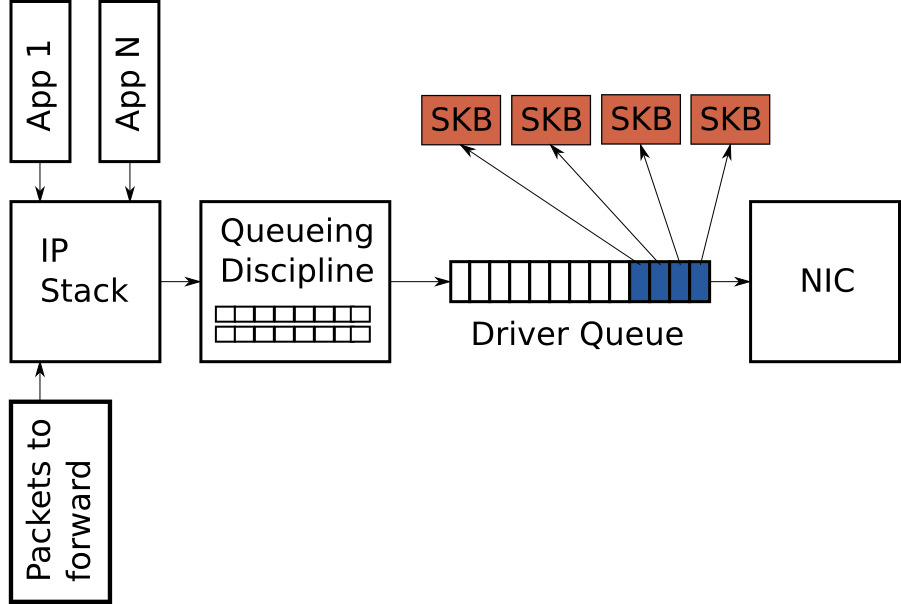
\includegraphics[width=0.8\textwidth]{figures/linux_networking.png}
    \caption{Simplified high level overview of the queues on the transmit path of the Linux network stack \cite{danQueueingLinuxNetwork2013}}
    \label{fig:linux_network}
\end{figure}

